\documentclass[../../ASSD_TP1_G7.tex]{subfiles}
\begin{document}
\chapter*{Entorno de simulaci\'on}
Para realizar la simulación se utilizo el programa GNU radio, de licencia libre. El modo de trabajo en dicho programa es similar al de symulink. Consta en bloques con funciones predefinidas y se unen a  través de cables. Ademas dicho programa permite generar una gui con los mismos bloques.
\par El programa que se realizo es el siguiente:

\begin{figure}[H]
\centering
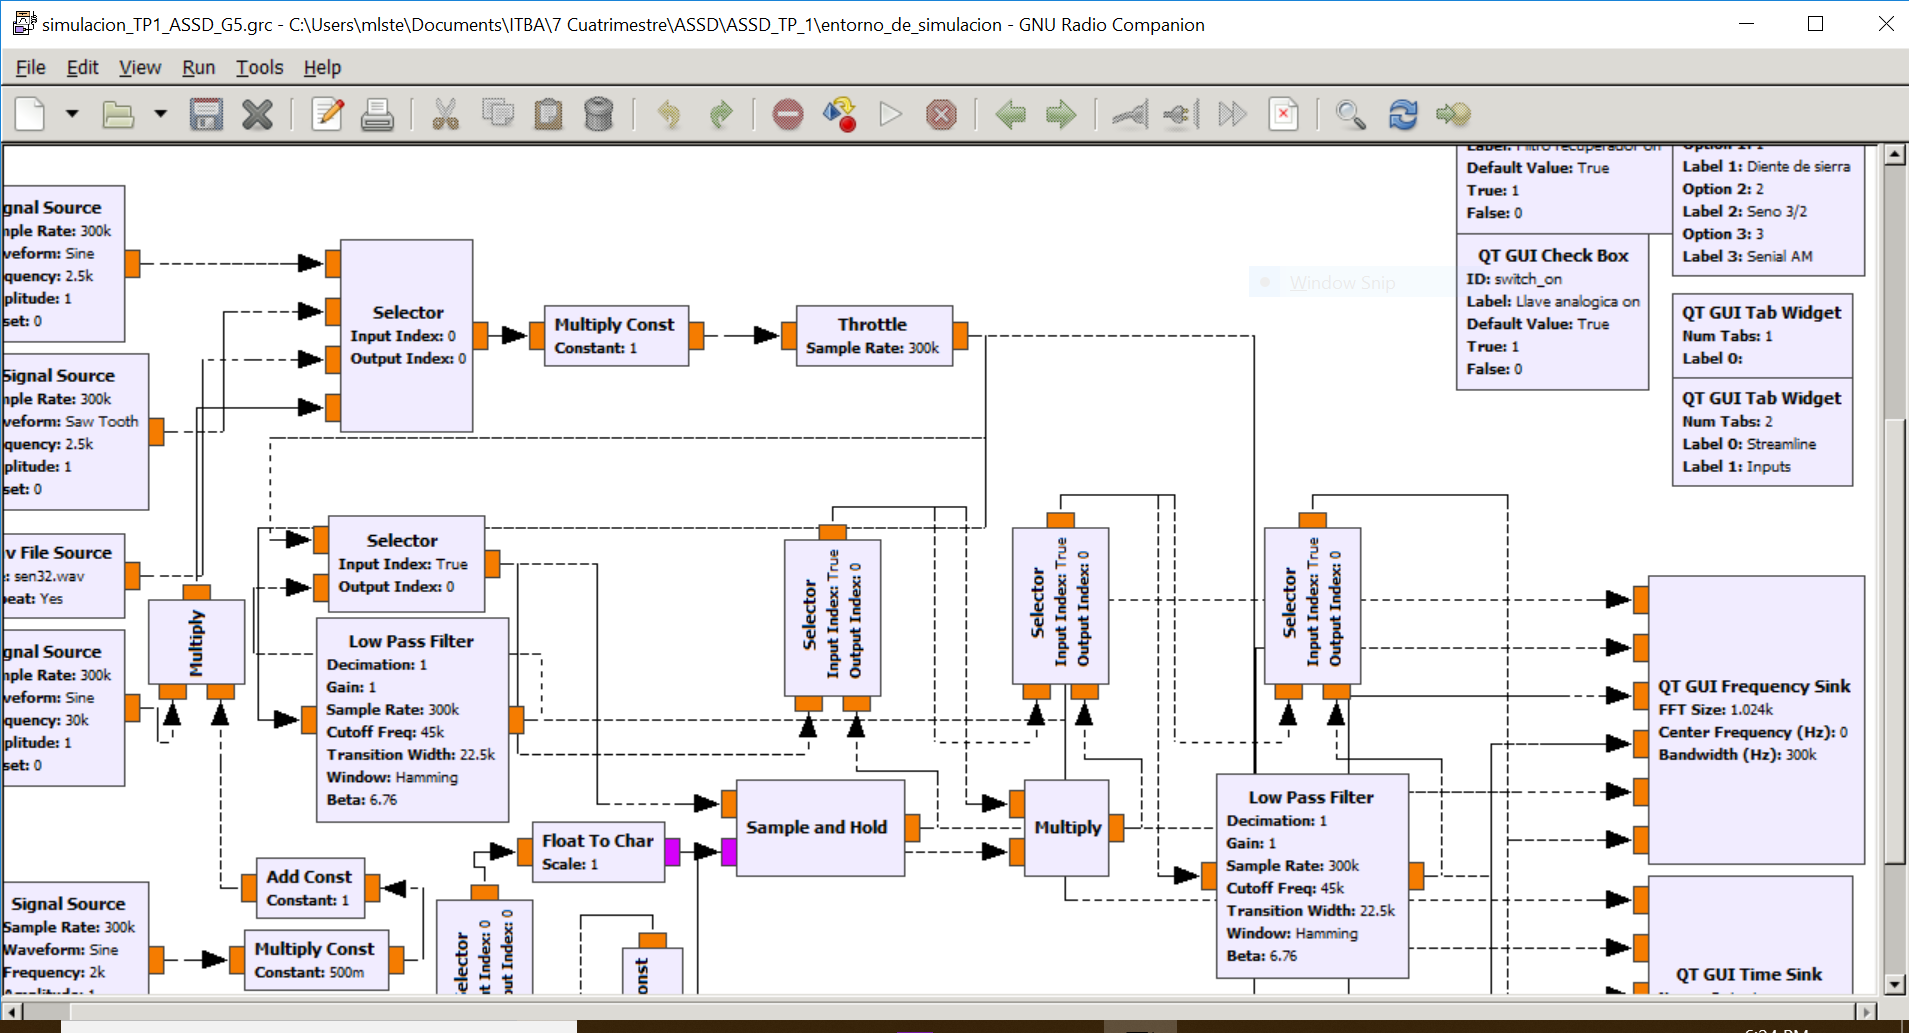
\includegraphics[width=0.75\textwidth]{figures/fig2.png}
\caption{Programa creado en GNU radio}
\end{figure}

\begin{figure}[H]
\centering
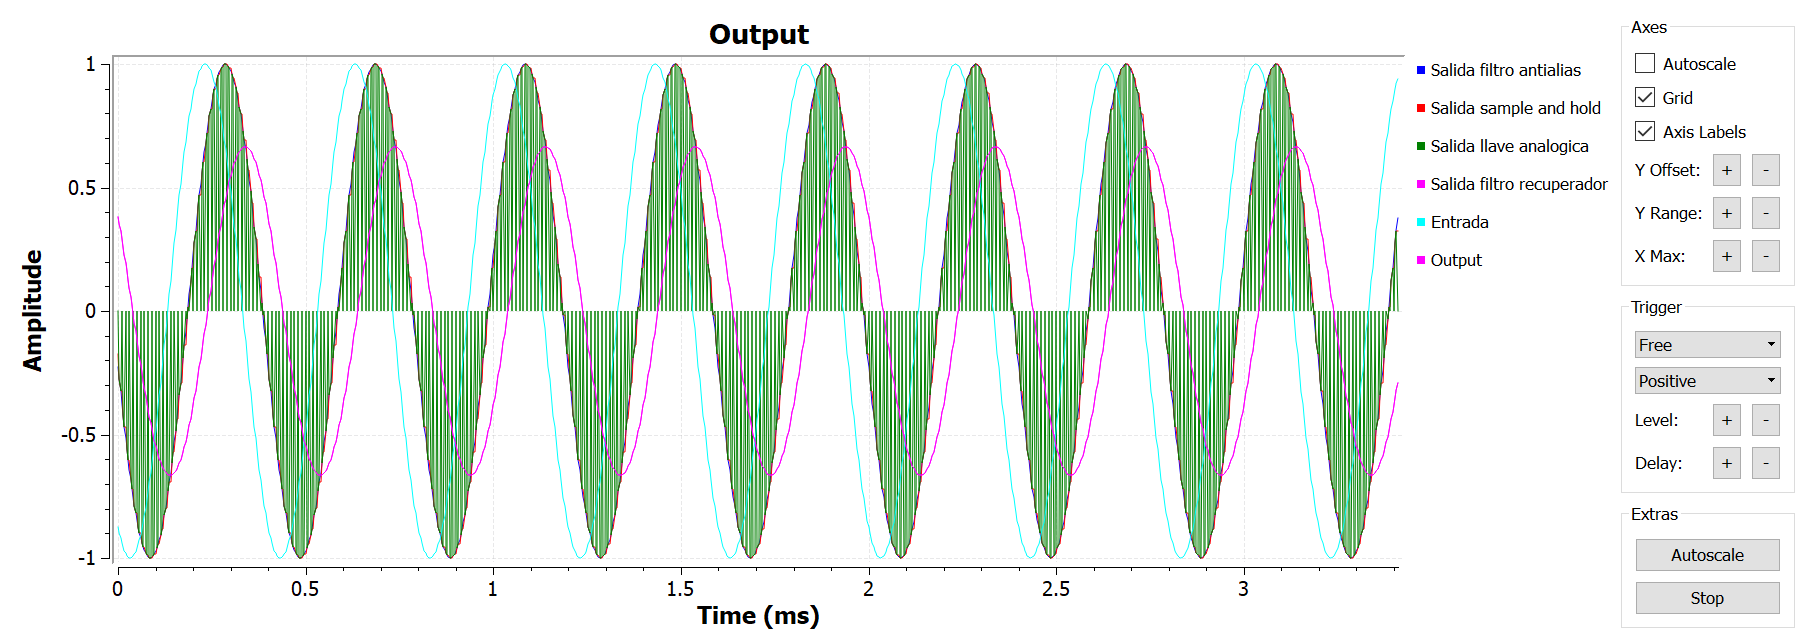
\includegraphics[width=0.75\textwidth]{figures/fig3.png}
\caption{GUI resultante}\label{fig:gui}
\end{figure}

El link de descarga de gnu radio es http://www.gcndevelopment.com/gnuradio/downloads.htm

\end{document}
